%--------------------
\subsection{粘土含水系モデルとメソMDシミューレションの条件}
本研究において組織構造解析に用いる2種類の粘土含水系メソMDモデル(モデル1と2)を
図\ref{fig:fig1}と図\ref{fig:fig2}示す。
これらの図は、粘土分子の初期状態(時刻$t=0$)における分布と、 粘土分子幅(粒径)のヒストグラムを示している。
いずれのモデルも周期構造を仮定し,粘土分子の初期配置を示した図には,
周期構造のユニットセルが破線で示されている.
2つのモデルの主たる違いは、粒径分布にありそれぞれのモデル分子数と粒径は
正規分布によって以下のように設定している。
\begin{itemize}
\item
モデル1
	\begin{itemize}
		\item 粘土分子数: 80
		\item 粗視化粒子数: 3,194
		\item 平均粒径 (標準偏差): 40 (10)[{\rm nm}]
	\end{itemize}
\item
モデル2
	\begin{itemize}
		\item 粘土分子数: 80
		\item 粗視化粒子数: 3,237
		\item 平均粒径 (標準偏差): 50(27)[{\rm nm}]
	\end{itemize}
\end{itemize}
これらの数値から明らかなように、モデル2はモデル1に比べて粒径分布の分散が大きく設定されている。
初期状態でのユニットセルのサイズは、200$\times$200[nm]の正方形とし、1[ns]の間にユニットセルを
等方的に65\%圧縮する。その結果、最終的には70$\times$70[nm]の正方形ユニットセルに、約80の粘土分子が
充填された組織構造が得られる。
なお、粘土分子は全て初期状態では二層膨潤に相当する水和水を持つものとする。ただし、
圧縮の過程において、近接する粗視化粒子間では粒子径のポテンシャルエネルギーが下がる場合には、
水和水の移動が生じることを許容するモデルを用いる。そのため、最終的にえられた組織構造において、水分
分布は一様でなく、必ずしも平均的に二層膨潤状態が維持される保証はない。圧縮は等温条件で進め、
系の温度は,粗視化粒子の運動エネルギーを各時間ステップでスケーリングすることで一定値を保つように
制御した.
%--------------------
\begin{figure}[h]
	\begin{center}
	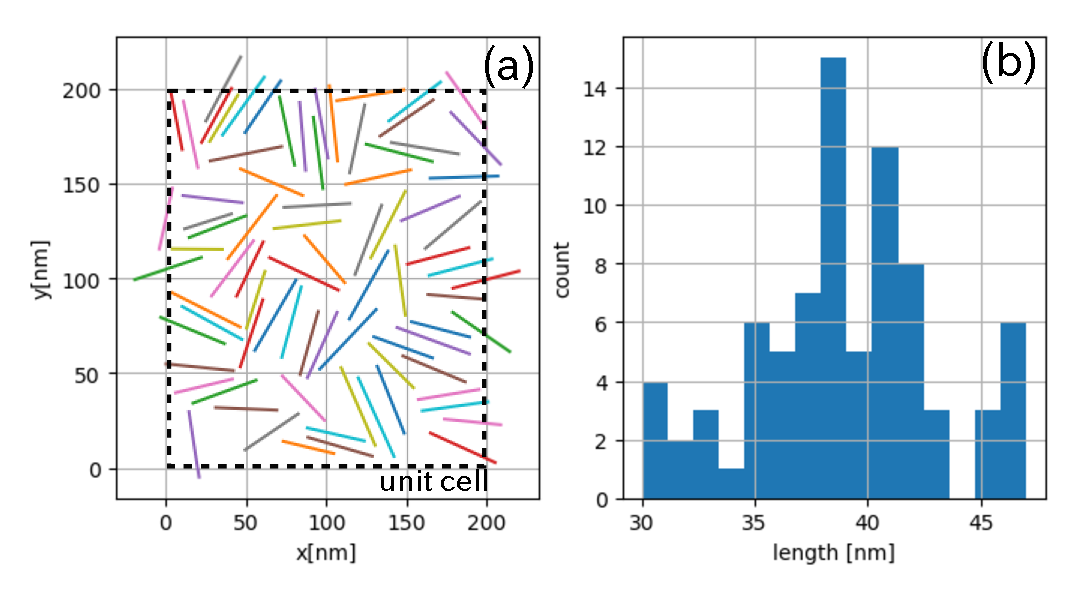
\includegraphics[width=0.8\linewidth]{Figs/fig1.eps} 
	\end{center}
	\caption{
		メソスケールMD解析モデル1. (a)粘土分子の初期分布.(b)粘土分子幅のヒストグラム. 
	} 
	\label{fig:fig1}
\end{figure}
%--------------------
\begin{figure}[h]
	\begin{center}
	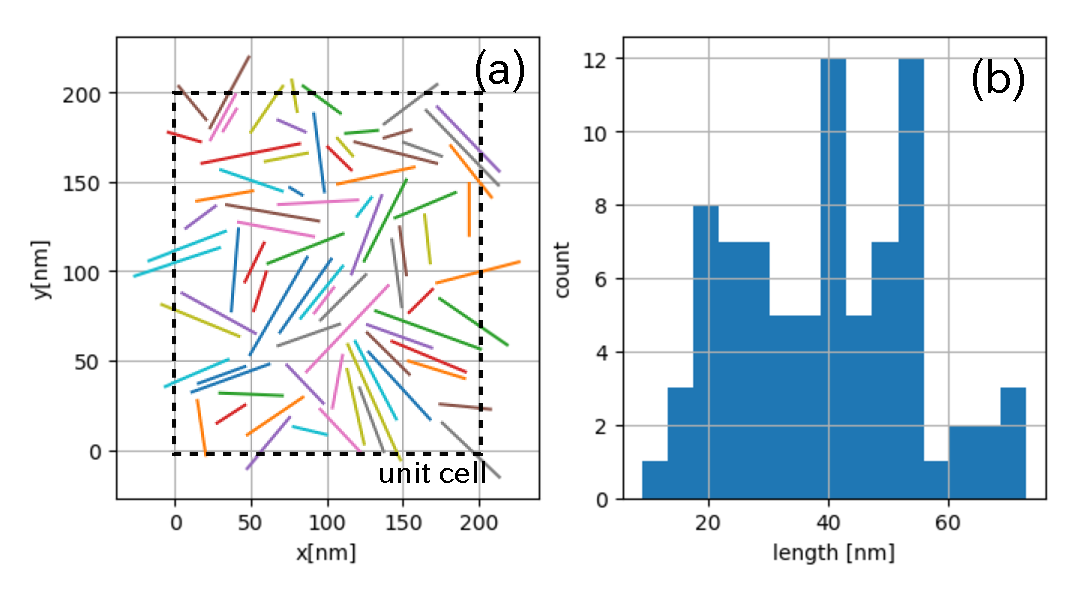
\includegraphics[width=0.8\linewidth]{Figs/fig2.eps} 
	\end{center}
	\caption{
		メソスケールMD解析モデル2. (a)粘土分子の初期分布.(b)粘土分子幅のヒストグラム. 
	} 
	\label{fig:fig2}
\end{figure}
%--------------------
\subsection{圧縮凝集過程のシミュレーション結果}
図\ref{fig:fig3}と図\ref{fig:fig4}に,上記のモデルと計算条件で行ったメソMD解析の結果を示す。
これらの図は、粘土分子分布のスナップショットを0.2ns毎に示したもので,ユニットセルの等温圧縮に
よる粘土分子の凝集挙動を示している。いずれのモデルでも、比較的早い段階から、近接する粘土分子が
積層構造を作るが、積総数はあまり大きくならない。また、積層した分子の間に残された大きな間隙が、
ユニットセルの圧縮に伴い、次第に縮小されて最終的にはほとんど消失する様子が見られる。
これらの結果では、2つのモデルにおいて粘土分子の配置は途中段階でも圧縮終了後も当然互いに異なるが、
凝集挙動や最終的にえられた組織構造に本質的な差があるかどうかは明らかでない。
しかしながら、このようにして得られた組織構造を次節で述べる方法によって処理し、X線回折パターン等の形で
比較すると、2つの組織構造モデルには有意な差があることが明らかとなる。
\begin{figure}[h]
	\begin{center}
	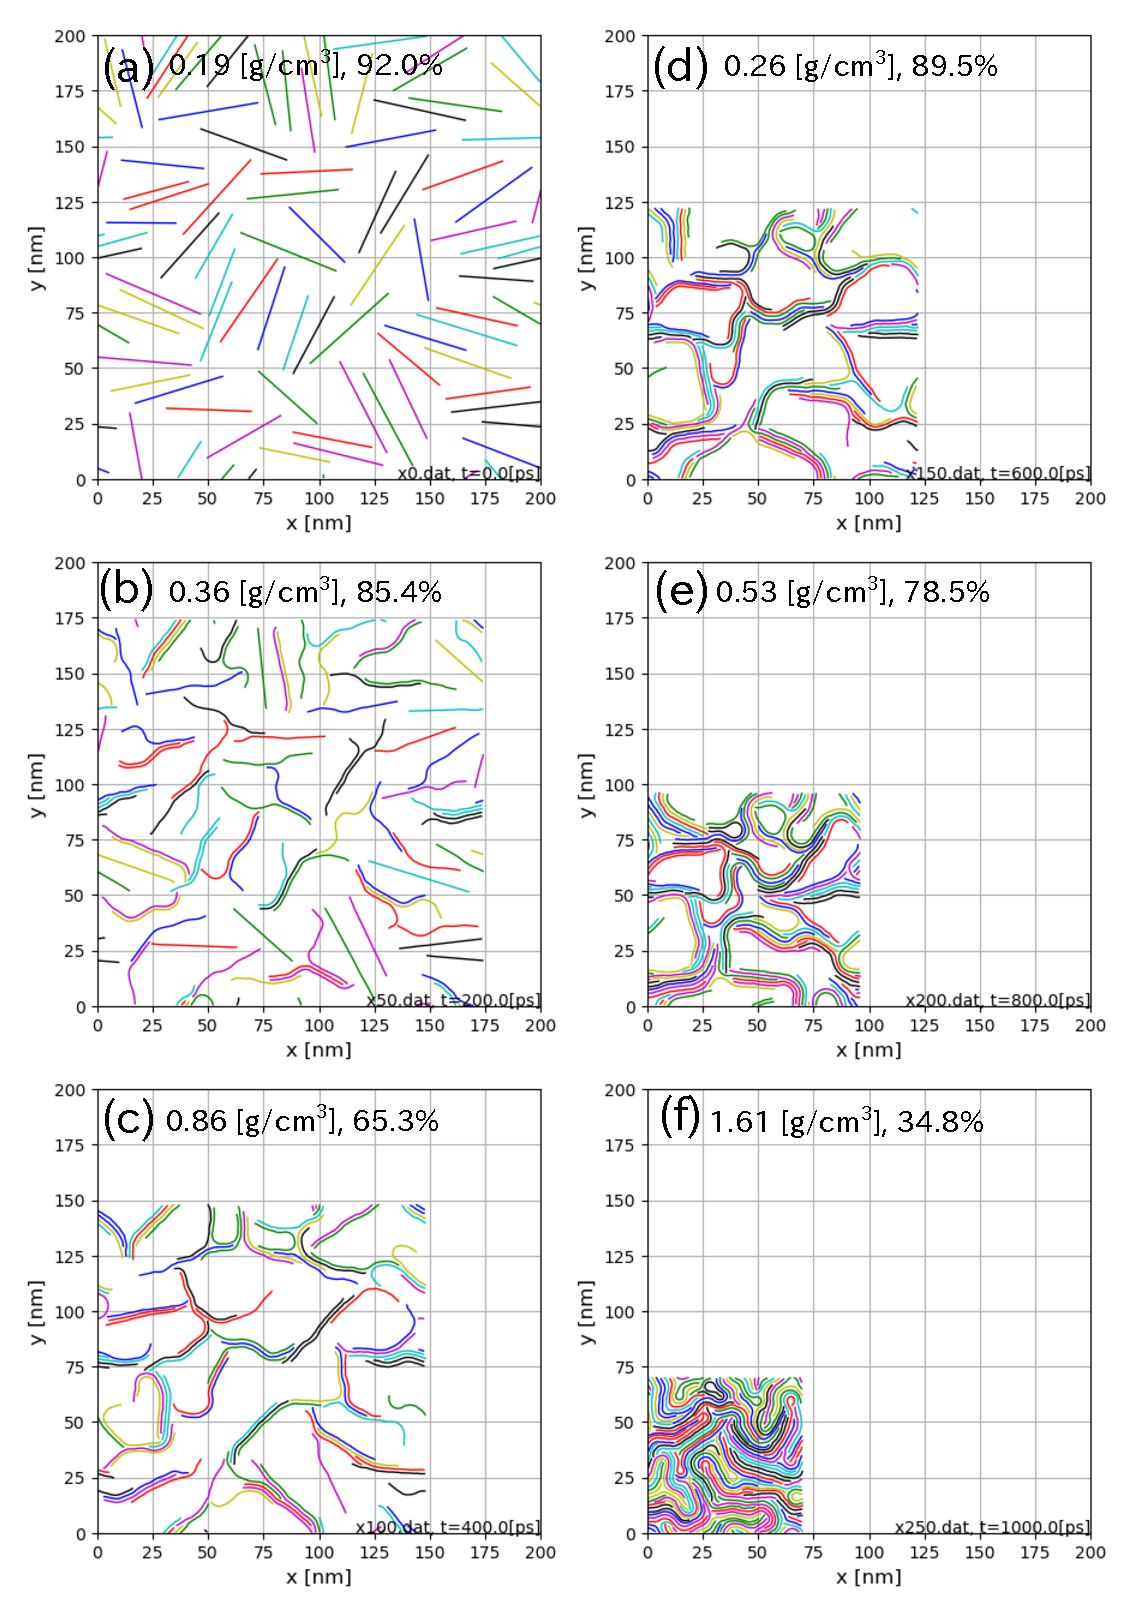
\includegraphics[width=1.0\linewidth]{Figs/fig3.eps} 
	\end{center}
	\caption{
		ユニットセルの圧縮に伴う粘土分子の凝集挙動(モデル1).
	} 
	\label{fig:fig3}
\end{figure}
%--------------------
\begin{figure}[h]
	\begin{center}
	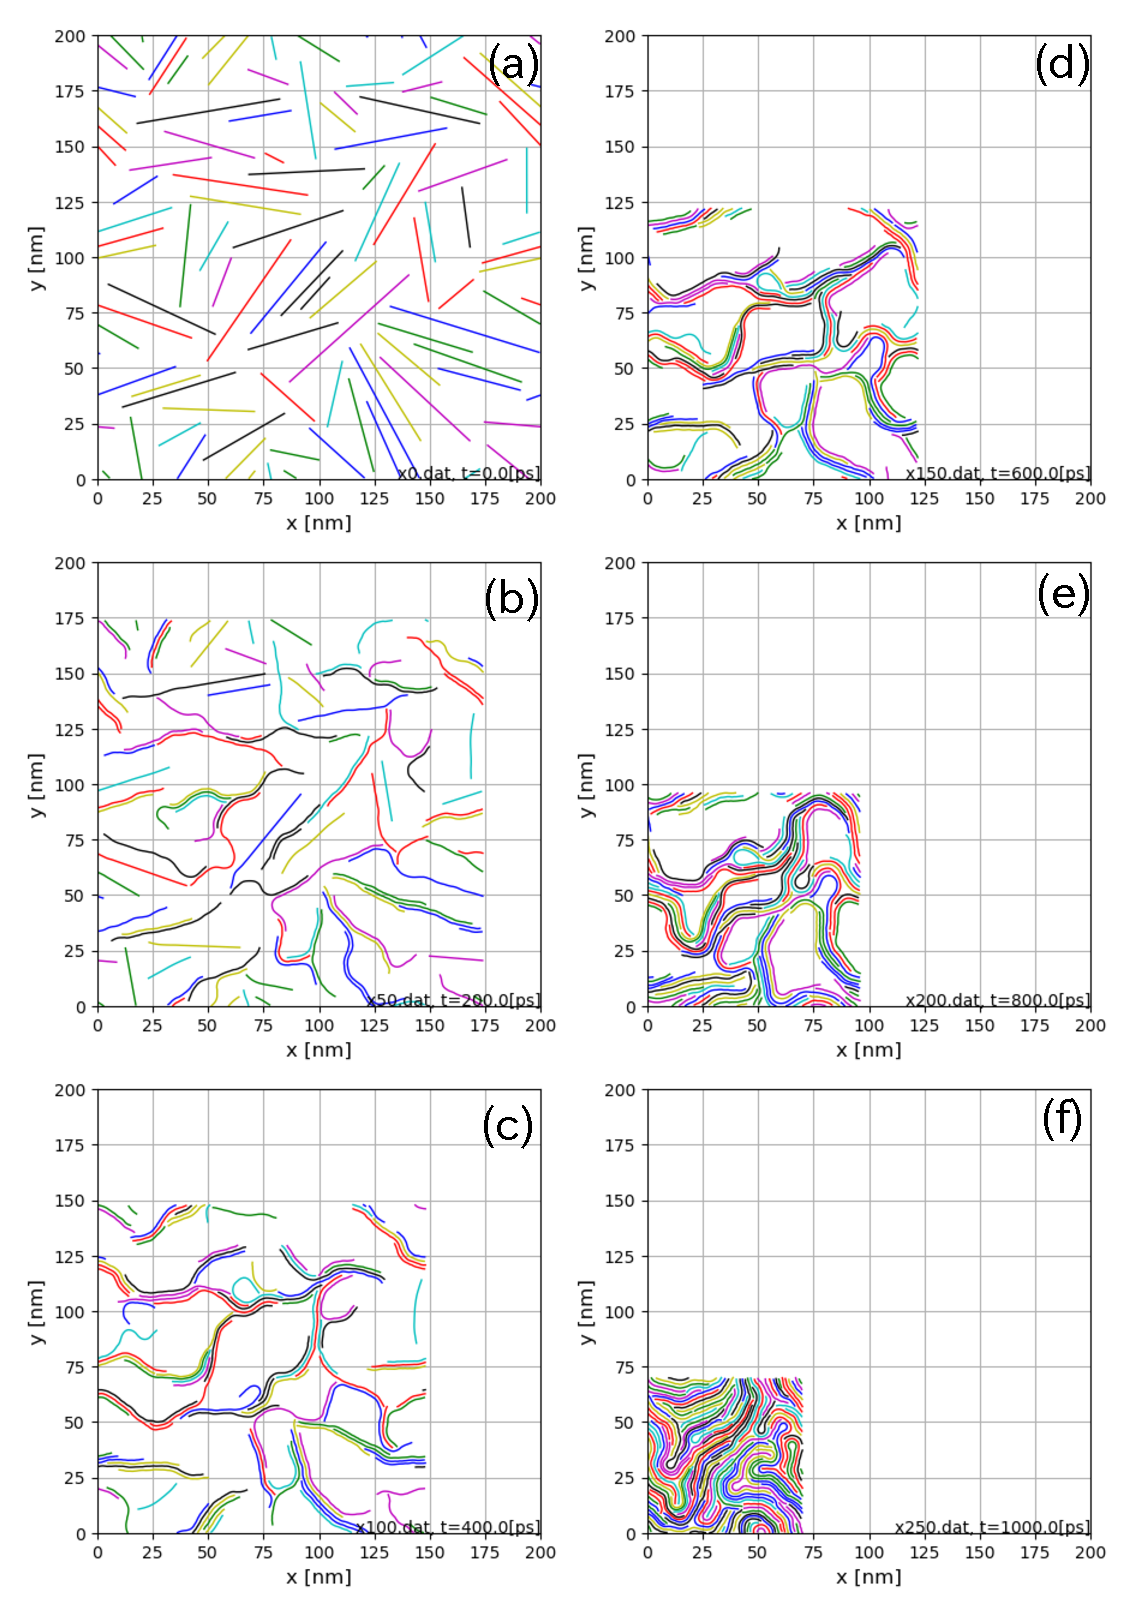
\includegraphics[width=1.0\linewidth]{Figs/fig4.eps} 
	\end{center}
	\caption{
		ユニットセルの圧縮に伴う粘土分子の凝集挙動(モデル2).
	} 
	\label{fig:fig4}
\end{figure}
%--------------------
